\section{Barium fluoride characteristics}

The existence of the very fast scintillation component in BaF$_2$ makes this crystal an attractive candidate for high rate applications such as the Mu2e calorimeter, in both its initial and possible upgrade phases. The  BaF$_2$ scintillation spectrum is shown in Figure~\ref{fig:spectrum}.  BaF$_2$ was thoroughly investigated as a candidate for the calorimeter of the GEM detector at the SSC\cite{Zhu:1992pm} more than two decades ago, and has, in fact, been employed in the TAPS experiment\cite{Novotny:1998bj} at Mainz, which does not have a magnetic field. For Mu2e to make full use of the high rate capability afforded by the fast decay time component at 220 nm, however, requires a means of rejecting the much more intense slow component at 300 nm with a readout device that can operate in a 1T magnetic field.   Solar blind photomultipiers have adequate quantum efficiency at 220 nm, and some rejection at 300 nm, but are not suitable for use in a magnetic field.

\begin{figure}[h!]
\centering
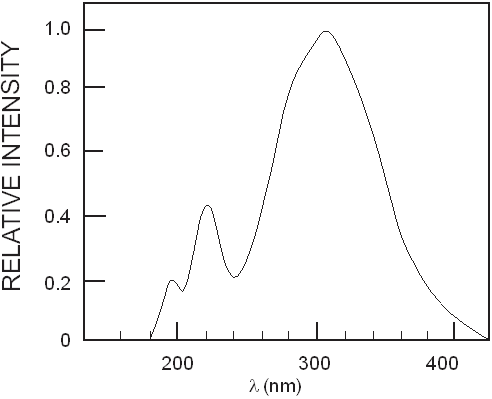
\includegraphics[width=0.9\linewidth]{Figures/spectrum.png}
\caption{The  BaF$_2$ fast scintillation component at 220 nm comprises $\sim$15\% of the light, the slow component at 300nm, $\sim$ 85\%}
\label{fig:spectrum}
\end{figure}

There are approaches to making use of the fast 220 nm component of BaF$_2$: reducing the size of the 300 nm component through doping and/or finding a suitable readout device that is insensitive to the slow component while retaining adequate quantum efficiency for the fast component. It is possible to reduce the 300 nm emission component without too much effect on the 220 nm component by doping with rare earths such as lanthanum\cite{woody:1989}, but this is not a large enough reduction to solve the problem at hand. We have begun a study of this type of doping, mainly aimed at understanding the radiation hardness of dope BaF$_2$ crystals.

Our main focus has been on developing UV sensitive solid state photosensors. There are commercial devices with extended UV response, but no large area devices that can discriminate between the wavelengths of the fast and slow components of BaF$_2$ emission. We have thus formed a Caltech/JPL/RMD collaboration to develop such a device.

